%/////////////////////////////////////////////////////////////////////////////
%
% Definition des Dokuments
%
%/////////////////////////////////////////////////////////////////////////////
\documentclass[
11pt,				% Schriftgröße
a4paper,			% Seitengröße
DIV12,		     	% Satzspiegel
liststotoc,			% Inhalsverzeichnis in Inhaltsverzeichnis
bibliography=totoc, % Quellenverzeichnis in Inhaltsverzeichnis
listof=entryprefix, % Abbildungsverzeichnis in Inhaltsverzeichnis
listot=entryprefix, % Tabellenverzeichnis in Inhaltsverzeichnis
appendixprefix=true,
pointlessnumbers,
%	DIV=calc,		% Satzspiegel autom. berechnen, widerspricht sich mit vorherigem
%	twocolumn,		% Zweispaltiger Text
	oneside,		% Doppelseitig, während dem Arbeiten ausschalten, dann besser zum arbeiten, für digitale Variante auch ausschalten, 
%	BROC=10mm		% Bindeausgleich, Achtung links oder rechts anpassen
]{scrbook}

% Zeilenabstand
\usepackage{setspace}
\usepackage{dirtree}
% Absatzeinrückung und -abstand
\parindent 	= 0pt
\parskip 	= 6pt

% Dateicodierung
\usepackage[utf8]{inputenc} 

% Spracheinstellung
\usepackage[ngerman]{babel}
\usepackage[ngerman]{translator}

%Besondere Trennungen
\hyphenation{De-zi-mal-tren-nung}

% Zeichencodierung
\usepackage[T1]{fontenc}
\usepackage{titlesec}

% Schriften einstellen
\usepackage{lmodern}		%Vektorschrift, keine Pixel
\usepackage{microtype}		%Verbessert microtypographie, Verbessert auch warnings 	(overfull boxes)
\renewcommand{\familydefault}{\sfdefault} 	% {1}Standard Schrift, {2}entfernt Serifen, 													Schrift dann ähnlich Calibri
\usepackage{sansmath}		% Mathemodus ohne Serifen
%\sansmath					% Mathemodus aktivieren

\setcounter{secnumdepth}{3}
\setcounter{tocdepth}{3}

% Bilder einbinden
\usepackage{graphicx}
\usepackage{subfigure} 
\graphicspath{{Bilder/}}  % können mehrere Pfade eingebunden werden, von aktuellen Dokument ausgehend


% Dynamisch verlinktes Dokument
\usepackage[%pdfborder={0 0 0 }, 
colorlinks = true,
linkcolor = blue,
pdftitle={Titel der Abschlussarbeit},
pdfsubject={},
pdfauthor={Euer Name},
pdfkeywords={},	
]{hyperref}		%[]Art und Weise für die Anzeige


%------------- Literatur ------------------------------------
\bibliographystyle{unsrt}

\usepackage{color}
\definecolor{middlegray}{rgb}{0.5,0.5,0.5}
\definecolor{lightgray}{rgb}{0.8,0.8,0.8}
\definecolor{orange}{rgb}{0.8,0.3,0.3}
\definecolor{yac}{rgb}{0.6,0.6,0.1}
\usepackage{listings}
 \lstset{
	language=C++,
	basicstyle=\footnotesize,
	keywordstyle=\color{blue}\ttfamily,
	stringstyle=\color{red}\ttfamily,
	commentstyle=\color{green}\ttfamily,
	morecomment=[l][\color{blue}]{\#},
	backgroundcolor=\ttfamily\color{white},
	frame = single 
}

%--------------Große Tabellen---------------------------------------
\usepackage{longtable}
%------------------------Mathe----------------------------
\usepackage{amssymb}
\usepackage{nicefrac}
\usepackage{amsfonts}
\usepackage{amsmath}
%-----------------------------------------------------------


%Befehle von Klaus
\newcommand{\x}{\mathbf{x}}
\newcommand{\y}{\mathbf{y}}
\newcommand{\A}{\mathbf{A}}
\newcommand{\B}{\mathbf{B}}
\newcommand{\C}{\mathbf{C}}
\newcommand{\PP}{\mathbf{P}}
\newcommand{\tp}{^{\mathrm{T}}}
\newcommand{\mat}{\boldsymbol}
\newcommand{\xxi}{\boldsymbol{\xi}}

%------------- Definition der Titelseite ---------------------

\title{Implementierung eines Frameworks für generische Flugzeugsimulationen in C++}

\author{Abschlussbericht für das Modul Effizient programmieren I \& II \\
	von \\
	Jan Olucak   }

%\label{
\publishers{durchgeführt am \\
	Institut für Aerodynamik und Gasdynamik \\
	der Universität Stuttgart \\
	[5ex]
	Stuttgart, im Juli 2018}

\date{}

% entweder erste Spalte fett oder Trennstrich, nicht beides

\usepackage{epsf}


%--------------- Kopf und Fusszeile --------------
\usepackage{scrpage2}
\pagestyle{scrheadings}
\clearscrheadfoot
\ifoot{}
\ofoot{\pagemark}

\automark[section]{chapter}
\ihead{\headmark}

\setheadsepline{0.2pt}
\usepackage{caption}
\usepackage{graphicx}
%\renewcommand{\thechapter}{\arabic{chapter}}
%\renewcommand{\thesection}{\arabic{section}}
%\usepackage{titlesec}
%------------------Hier beginnt das Dokument---------------------------------
%-----------------------------------------------------------------------------
%-----------------------------------------------------------------------------
\begin{document}
	
\maketitle							% fügt Titel in Dokument ein

\pagenumbering{Roman}
\pagestyle{empty}



\pagestyle{empty}
\tableofcontents
\newpage 
\pagestyle{scrheadings}
\setcounter{page}{1} 
\pagenumbering {Roman} 
\listoffigures
\newpage
\listoftables
\newpage

\renewcommand{\chapterpagestyle}{scrheadings}
\newpage
\include{Abbkuerzungsverzeichnis}
\newpage
\include{Symbolverzeichnis}

\pagestyle{scrheadings}
\setcounter{page}{1} 
\pagenumbering {arabic} 

% ab hier Zeilenabstand 1,5
\onehalfspacing
\renewcommand{\chapterpagestyle}{scrheadings}

\chapter{Problemstellung}
\section{Ausgangslage}
Der Prozess des Flugzeugentwurfs erstreckt sich über mehrere Schleifen in denen das Flugzeug immer detaillierter Ausgearbeitet wird. Um das Leistungsvermögen früh im Entwicklungsprozess zu beurteilen, können numerische Simulationen genutzt werden. Zum einen werden mathematische Modelle benötigt, um das physikalische Verhalten von spezifischen Domänen des Flugzeuges abzubilden, zum anderen werden Parameter benötigt, um besagte Modelle zu beschreiben. Viele Parameter sind erst im Laufe des Entwurfsprozesses verfügbar. Um das Flugverhalten dennoch abzubilden, wird eine Simulation mit verschiedenen Ausbaustufen und Fehlermodellen benötigt. \\
Aus den meisten Ingenieursanwendungen ist MATLAB nicht mehr wegzudenken. Grund hierfür ist das breite Anwendungsspektrum und die Vielzahl an zusätzlichen Toolboxen. Dabei handelt es sich um eine proprietäre Programmiersprache die auf dem jeweiligen Rechner interpretiert wird. Trotz der vielseitigen Anwendungsmöglichkeiten benötigt MATLAB für komplexere Anwendung eine größere Laufzeit, im Vergleich zu Programmiersprachen, welche direkt in Maschinensprache übersetzt werden. Die Laufzeit ist mitunter einer sehr kritische Größe bei der Nachweisführung und Leistungsrechnung. 
\section{Kurzvorstellung Programm Aircraft Designer}
In der Arbeit nach  \cite{Olucak.15.02.2017} wurde eine MATLAB basierendes Programm entwickelt, mit dessen Hilfe Simulationsmodelle für Flugzeuge modelliert werden können. Die fertigen Modelle werden sowohl in Text-Files, als auch in MATLAB spezfischen .mat-files gespeichert. Um die Modelle zu verifizieren wurde zudem eine Simulation mit 6 Freiheitsgraden implementiert. Das Programm Aircraft Designer kann jederzeit um weitere Methoden ergänzt werden, um so den Entwurfsprozess fortzusetzen. 
\section{Zielsetzung}
 

\chapter{Aufbau der Simulation}
\section{Grundidee des Simulation-Frameworks}
\subsection{Beispiel Navigation-Klasse }
\section{Ablauf der Simulation}


\chapter{Durchführung der Implementierung}
\section{Implementierungs-Prozess}
Für die Verifikation des Frameworks wird die Matlab-Simulation nach \cite{Olucak.15.02.2017} verwendet. Da es hier lediglich um eine Konvertierung des Codes handelt, werden die mathematischen Modelle nicht explizit erklärt. Vielmehr wird das Vorgehen der Implementierung erläutert, um zu zeigen, wie Programm effizient entwickelt wurde. Gleiches gilt für die Implementierung der Simulationswerkzeuge.\\
 Die Simulations-Umgebung wurde sukzessive aufgebaut. Es wurde stets darauf geachtet, dass nach der Implementierung einer Funktion nach möglich direkt getestet wurde. Erst mit der nachgewiesenen Funktionalität, wurde der nächste Schritt im Prozess durchgeführt. In Abbildung \ref{fig:ImpProzess} wird dieser Prozess dargestellt.
\begin{figure}[h]
	\includegraphics[width=1.0\linewidth]{ImpProzess.PNG}
	\label{fig:ImpProzess}
	\caption{Flussdiagramm des Implementierungs-Prozess}
\end{figure}
\section{Simulationswerkzeuge}
Unter Simulationswerkzeugen sind Funktionen zu verstehen, die in allen Teilen des Simulations-Frameworks vorkommen. Dies umfasst beispielsweise das Einlesen und Schreiben von Simulationsparametern oder mathematische Funktionen wie Integration oder Interpolation. Es ist offensichtlich, dass besagte Funktionen als erstes implementiert werden müssen, damit die Module im späteren Verlauf auf diese zurückgreifen können. Diese Werkzeuge wurden eigens in das Modul \textbf{Tools} implementiert. Auch die in \ref{sec:OSBib} beschriebenen Bibliotheken fallen unter diese Werkzeuge. Die implementierten Simulationswerkzeuge werden in Tabelle \ref{tab: SimWerk} zusammengefasst.
\begin{table}[h]
\centering	\begin{tabular}{lp{11cm}}
		\textbf{Funktion/Klasse} & \textbf{Kurzbeschreibung}\\
		 Constants & physikalische Konstanten\\\\
		 DataLogger & Klassen, um Parameter in ein Text-File zu schreiben\\\\
		 LinearInterpolation & Ein- und zweidimensionale Interpolation bereitstellt\\\\
		 MatFileReader & Funktionen zum Einlesen von .mat-File\\\\
		 ODESolver & Templates für numerische Integration\\\\
		 readInData & Funktionen zum Einlesen von Parametern aus Text-Files\\\\
		 Transformation & Matrizen für Koordinaten-Transformation
	\end{tabular}
\label{tab: SimWerk}
\caption{Simulationswerkzeuge der generischen Flugzeugsimulation}
\end{table}
\newpage
\subsection{Unit-Tests}
Um sicherzustellen, dass die Werkzeuge korrekt implementiert wurden, wurden Unit-Test implementiert. Dazu wurde das in Visual Studio bereitgestellte Microsoft-Komponententest-Frameworks für C++ genutzt. Die Unit-Tests wurden in einen gleichnamigen Projektordner ausgelagert. An dieser Stelle werden nicht alle Test erklärt. Vielmehr soll das Test-Schema erläutert werden.\\ In dieser Arbeit wird das AAA-Schema  (Arrange, Act, Assert) nach \cite{Microsoft.2018}  genutzt. Dazu werden die Tests in die zuvor genannten Abschnitte aufgeteilt. Im einzelnen haben die Abschnitte folgende Bedeutung \cite{Microsoft.2018}: 
\begin{itemize}
	\item  \underline{Arrange} dient der Initialisierung des Tests. Die benötigten Objekte werden initalisiert und Parameter für den Testfall festgelegt.   
	
	\item  Innerhalb von \underline{Act} wird die zu testende Methode mit den zuvor definierten Testfall/Parametern aufgerufen.
	
	\item Im Abschnitt \underline{Assert} werden die Referenzwerte mit den Werten aus dem eigentlichen Test vergleichen. Wird eine Übereinstimmung festgestellt, erhählt der Testfall seine Bestätigung durch das Framework.
\end{itemize}
Die Referenzwerte wurden entweder selbst festgelegt (z.B. Einlesen eines Parameters) oder es wurde Matlab genutzt, um Referenzwerte zu generieren (z.B. Interpolation). \\
Nach \cite{TuxFamily.2018} handelt es sich bei eigen um eine vollständig getestete Bibliothek. Aus diesem Grund wird auf eine Unit-Tests verzichtet. Bei der auf \cite{Hulbert.2013} beruhenden MatFileReader-Klasse wird nur der selbst geschrieben Code getestet. Eine Außnahme bei den Unit-Test stellt das Header-File Constants, bei der lediglich physikalische und mathematische Konstanten hinterlegt sind. 

\section{Implementierung und Testen der Module}
In \ref{sec:AufbauModule} wurde bereits der Aufbau der Module erläutert und in \ref{sec:Ausbaustufen} die für die Simulation benötigten Module aufgelistet. Um die Simulation wie im Baukastenprinzip zusammenzusetzen, ist es erforderlich, dass jedes Teil-Modul korrekt funktioniert.\\
Die Schwierigkeit, die mit den Modul-Tests einhergeht, ist die Definition der Testfälle. Ziel ist es eine größtmögliche Code-Coverage zu haben, um zu garantieren, dass das Modul wie gewünscht funktioniert.Bei einigen Modulen ist das Testen nur bedingt oder  nur im Gesamtsystem-Test möglich. Dies betrifft beispielweise das \textbf{Autopilot} und \textbf{Guidance} Modul. Für beide Module werden Parameter von anderen Modulen benötigt. \\Eine weitere Problematik besteht bei den verschiedenen  Modellen der Ausbaustufen. Wie schon erwähnt, wird die 6 Dof-Simulation nach \cite{Olucak.15.02.2017} genutzt, um das Simulations-Framework zu testen. Somit liegen nur zu den dort verwendeten Modellen Referenzwerte vor. Für die Simulation mit 3 Freiheitsgraden liegt keine Referenz vor. Ähnlich verhält sich die 6 Dof-Simulation mit Fehlermodellen. Es liegen aktuell keine Modelle für Sensorik und Aktuatorik vor. Somit können an dieser Stelle keine Modul-Tests für die zusätzlichen Module erfolgen.
In Tabelle \ref{tab:modultests} werden die Module  und deren Testfälle aufgezeigt, für die ein Modul-Test in Betracht kommt.\\
\begin{table}[h]
\centering	\begin{tabular}{l p{12cm}}
		\textbf{Modul} & \textbf{Beschreibung Testfall}\\
		Atmosphere & Bei dem hier hinterlegten Modell  handelt es sich um die Standard-Atmosphäre von 1976.  Temperatur, Druck, Dichte und Schallgeschwindigkeit sind hierbei abhängig von der Flughöhe. Somit werden die zuvor beschriebenen Größen von 0-10000m berechnet und mit Daten der Standard-Atmosphäre verglichen.\\\\
		Aerodynamic & Hier wird ein Windtunnel bei konstanter Höhe simuliert. Es werden Machzahl, Anstellwinkel und Höhenruder-Winkel variiert. Es ist ersichtlich, dass nur die Längsbewegung betrachtet wird. Dies ist auf mangelnde Referenzwerte für die Seitenbewegung zurückzuführen. Ziel dieses Tests ist es die Polare des Flugzeuges abzufahren und mit den Matlab-Daten zu vergleichen. \\\\
		Autopilot &  Die Parameter für das Gain Scheduling werden eingelesen und die Zustände auf Arbeitspunkt (Trimmpunkt) initialisiert. Es wird überprüft, ob die Scheduling Parameter und Stellgrößen nach der Initialisierung mit denen aus Matlab übereinstimmen.\\\\
		Trajectory & Der Trajectory-Modul Test testet die korrekte Berechnung der Flugbahn. Hier wird die Matlab-Simulation simuliert. Im Anschluss können die Ergebnisse verglichen werden.
	\end{tabular}
\label{tab:modultests}
\caption{Auflistung der Modultests}
\end{table}
\newpage
Aufgrund der Einfachheit des aktuell hinterlegten Schub-Models (Engine-Modul) wurde auf einen Modul-Test verzichtet und der Nachweis über Code-Reading durchgeführt.
Es ist offensichtlich, dass das Trajektorien-Modul erst aufgebaut werden konnte, nachdem die dafür benötigten Module bereits erfolgreich getestet wurden.


\section{Verifikation des Simulations-Framework}


\chapter{Optimierung der Simulation}
\section{Grundlegende Rechnerdaten}
An dieser Stelle wird der Rechner und genutzte Tools, womit die Implemetierung durchgeführt wurde, kurz aufgezeigt. Die grundlegenden Daten des Rechners sind in Tabelle \ref{tab:Rechnerdaten} zusammengefasst.
\begin{table}[h]
	\centering	\begin{tabular}{l p{10cm}}
		\textbf{Eigenschaft} & \textbf{Beschreibung/Wert}\\
		Betriebssystem & Windows 10\\
		Prozessor & Intel(R) Core(TM) i7-6600U CPU @ 2.60GHz 2.81GHz\\
		RAM & 8 GB\\
		Systemtyp & 64-Bit 
	\end{tabular}
	\caption{Rechnerdaten}
	\label{tab:Rechnerdaten}
\end{table}\\
\section{Vergleich der Rechenzeit Matlab und C++}
\section{Code Optimierung}
\section{Parallelisierung}

\chapter{Schlussbetrachtung}
\section{Diskussion des Gesamtergebnis}
Eines der Ziele, ein generisches Simulations-Framework für Flugzeuge in C++ zu implementieren wurde dadurch erreicht, dass sämtliche Parameter aus Input-Files eingelesen werden und die Methoden sehr allgemein gehalten wurden. Durch den modularen Aufbau können die einzelnen Module jederzeit um weitere Klassen erweitert werden. Die Simulation selber kann über ein Input-File gesteuert werden, womit unterschiedliche Modelle und Ausbaustufen ausgewählt und simuliert werden können, ohne dass der Nutzer den Code selbst verändern muss. In Kapitel \ref{ch:opt} wurde die Performance Optimierung der Simulation erläutert. Das Ziel, die Rechenzeit gegenüber Matlab  zu verbessern und im Nachgang weiter zu optimieren wurde erfüllt, wie in Abbildung \ref{fig:optergeb} zu sehen ist. 
\begin{figure}[h]
	\centering
	\includegraphics[width=0.7\linewidth]{untitled}
	\caption{Vergleich der Rechenzeiten}
	\label{fig:optergeb}
\end{figure}\noindent\\
Durch die Kompilierung als Release, konnte nochmals ein erheblicher Performancegewinn erzielt werden. Quantitative ergibt sich dadurch eine Rechenzeiteinsparung von 97,2\% gegenüber Matlab und 90\% gegenüber dem optimierten C++ Code.
\section{Erweiterungsmöglichkeiten}
Das Simulationsframework kann aufgrund des modularen Aufbaus jederzeit um weitere Klassen ergänzt werden. Es wurde bereits erwähnt, dass die höchste Ausbaustufe derzeit noch keine Fehlermodelle der Subsysteme besitzt. Diese und auch andere Erweiterungen könnten in Zukunft implementiert werden. Derzeit werden die Unit- und Modultests nur manuell durchgeführt. Eine Automatisierung der Tests wäre denkbar.
\section{Fazit}
Die in dieser Arbeit gesetzten Ziele wurde mit Erfolg erfüllt. Die Verwendung von Polymorphie wird als sehr effektiv angesehen, um ein Programm modular aufzubauen und um Code zu sparen. Zudem haben sich die in \cite{Kessler.Sommersemester2017}  und \cite{Kessler.Wintersemester201718} vorgestellten Tools zur effizienten Programmierung bewährt. Die zusätzlich Codedokumentation erwies sich als zusätzliche Last und fordert eine gewisses Maß an Selbstdisziplin. Durch die Durchführung von Unit- und Modultests, konnte die Funktion einiger Methoden nachgewiesen werden. Dennoch ist es sehr schwierig die Tests so zu definieren, um eine große Codeabdeckung zu gewährleisten. Der Leistungsprofiler ist sehr empfehlenswert, um Schwachstellen im Code zu erkennen und nachträglich algorithmisch zu optimieren. Die Möglichkeit der Parallelisierung konnte in dieser Ausarbeitung aufgrund des physikalischen Hintergrunds der Simulation nicht genutzt werden. Zusammenfassend lässt sich sagen, dass dem Nutzer eine funktionsfähige effiziente Simulationsumgebung für Flugzeuge zur Verfügung gestellt wird. 



\setcounter{page}{1} 
\pagenumbering {Roman} 
\appendix 
\chapter{}
\addcontentsline{toc}{chapter}{Anhang} 
\section{Vergleich der Simulationsergebnisse}
Es werden die Ergebnisse der Simulationen aus C++ und Matlab gegenübergestellt. In \ref{fig:bahn} ist klar zu erkennen, dass kein Bahnregler vorhanden ist. In beiden Simulationen folgt das Flugzeug den Querbeschleunigungen. Im Weiteren werden die Zustandsgrößen der Längs- und Seitenbewegung dargestellt.\\
\label{sec:simerg}
 \begin{minipage}{0.49\linewidth} 	
	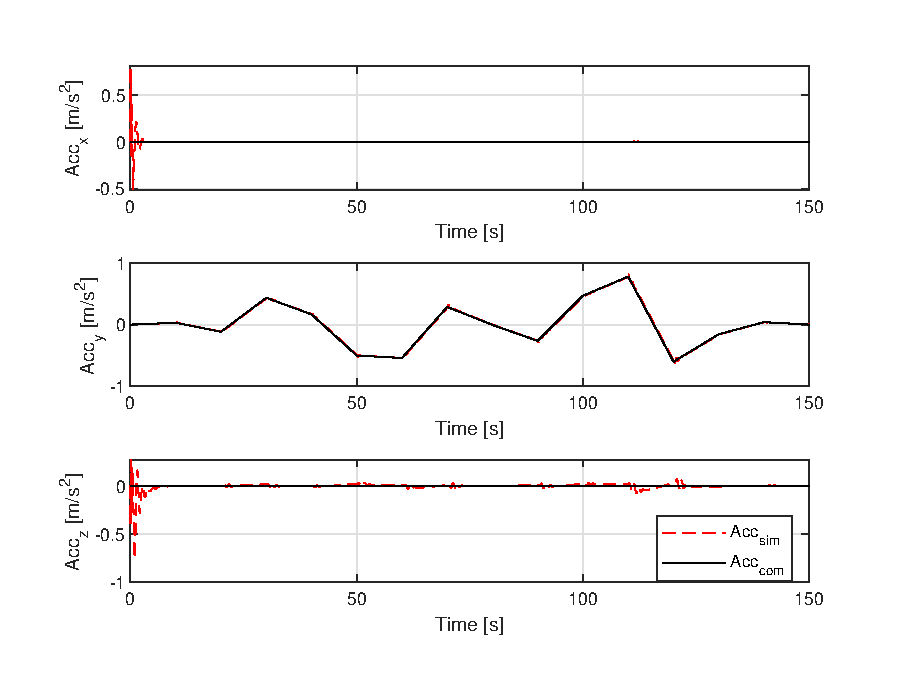
\includegraphics[width=1.0\linewidth]{querbeschleunigungen}
\end{minipage}
\begin{minipage}{0.01\linewidth}
	\hfill
\end{minipage}
\begin{minipage}{0.49\linewidth}
	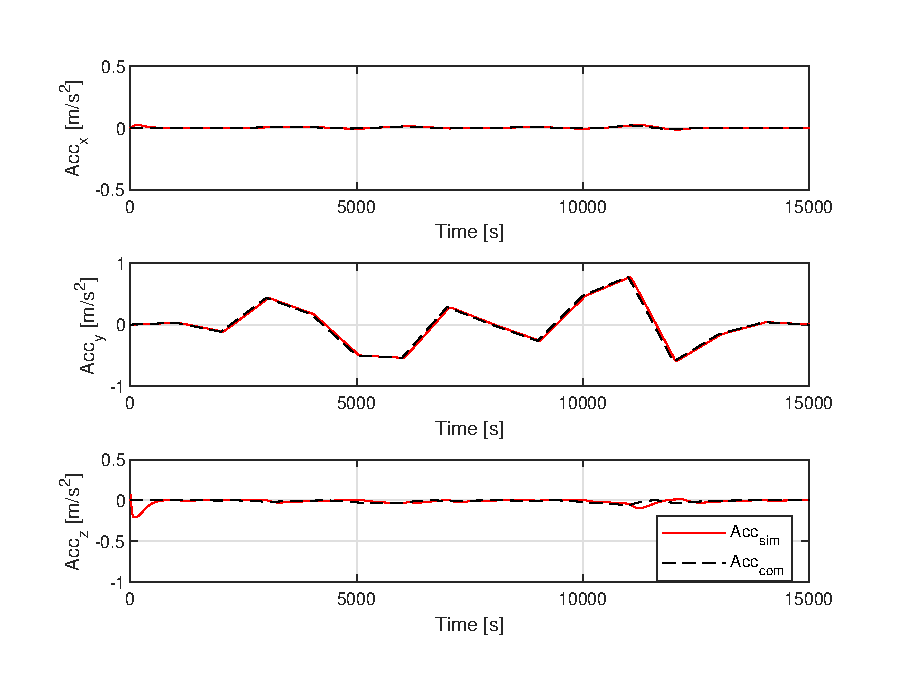
\includegraphics[width=1.0\linewidth]{matSim}
\end{minipage}
\captionof{figure}{Vergleich Querbeschleunigungen, links C++, rechts Matlab}\noindent\\
%
%
 \begin{minipage}{0.49\linewidth} 	
	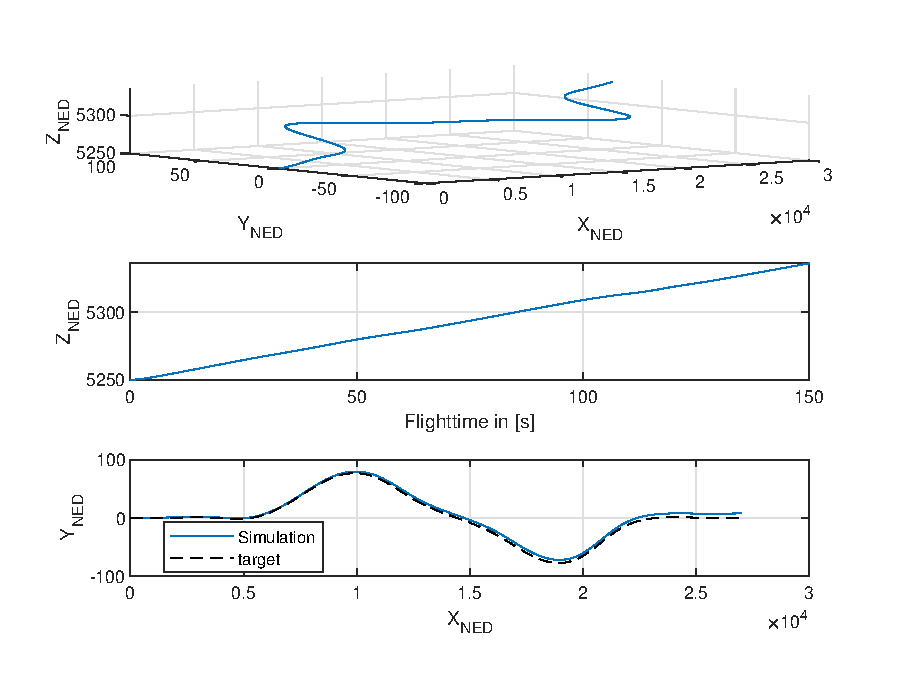
\includegraphics[width=1.0\linewidth]{trajectory}
\end{minipage}
\begin{minipage}{0.01\linewidth}
	\hfill
\end{minipage}
\begin{minipage}{0.49\linewidth}
	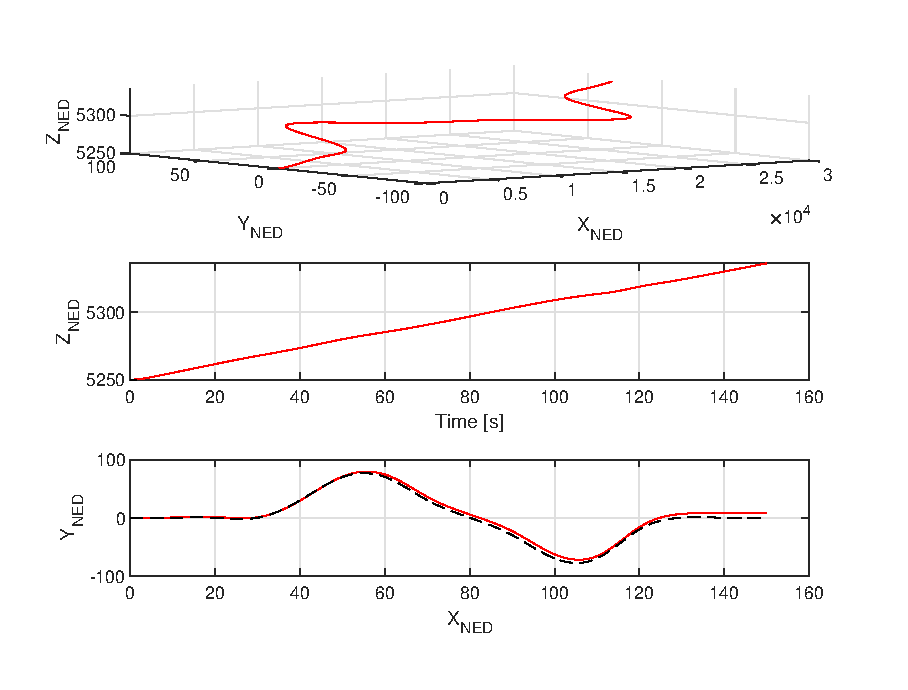
\includegraphics[width=1.0\linewidth]{trajectory_mat}
\end{minipage}
\captionof{figure}{Vergleich der Trajektorien, links C++, rechts Matlab}
\label{fig:bahn}\noindent\\
%
%
 \begin{minipage}{0.49\linewidth} 	
	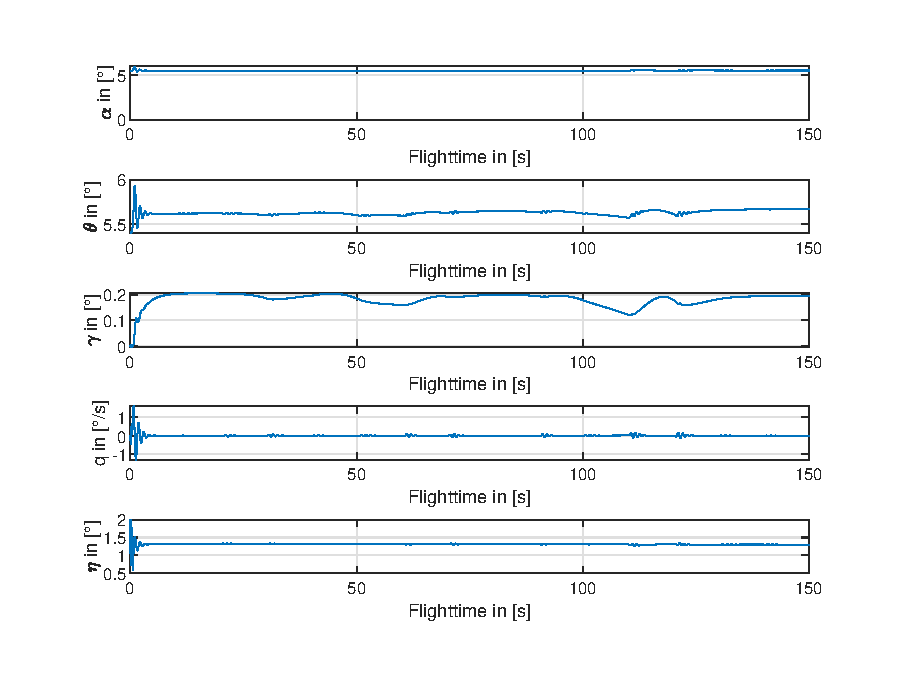
\includegraphics[width=1.0\linewidth]{pitch}
\end{minipage}
\begin{minipage}{0.01\linewidth}
	\hfill
\end{minipage}
\begin{minipage}{0.49\linewidth}
	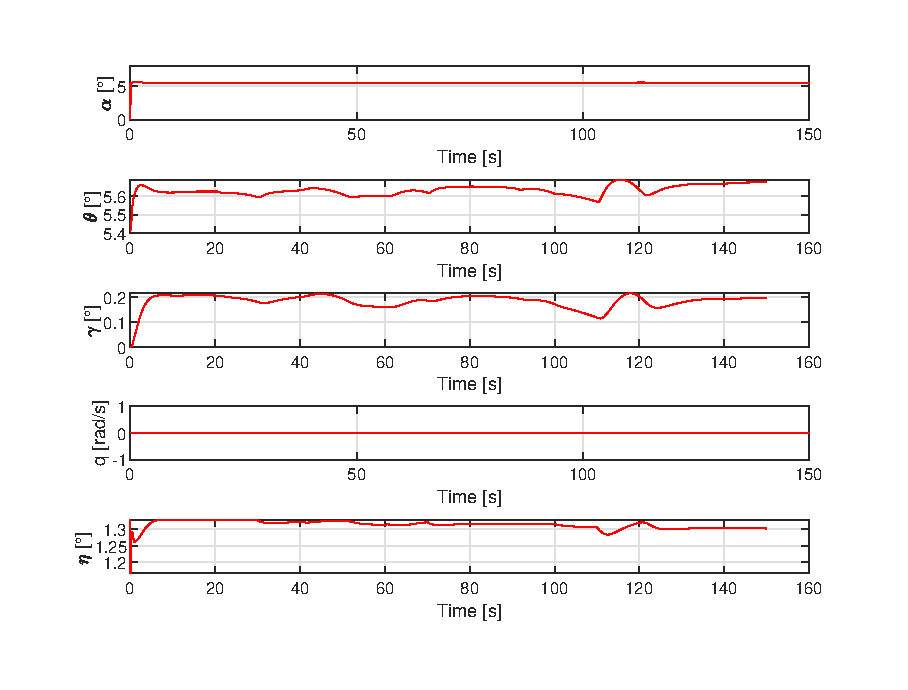
\includegraphics[width=1.0\linewidth]{pitch_mat}
\end{minipage}
\captionof{figure}{Vergleich der Längsbewegung, links C++, rechts Matlab}\noindent\\
%
%
\begin{minipage}{0.49\linewidth} 	
	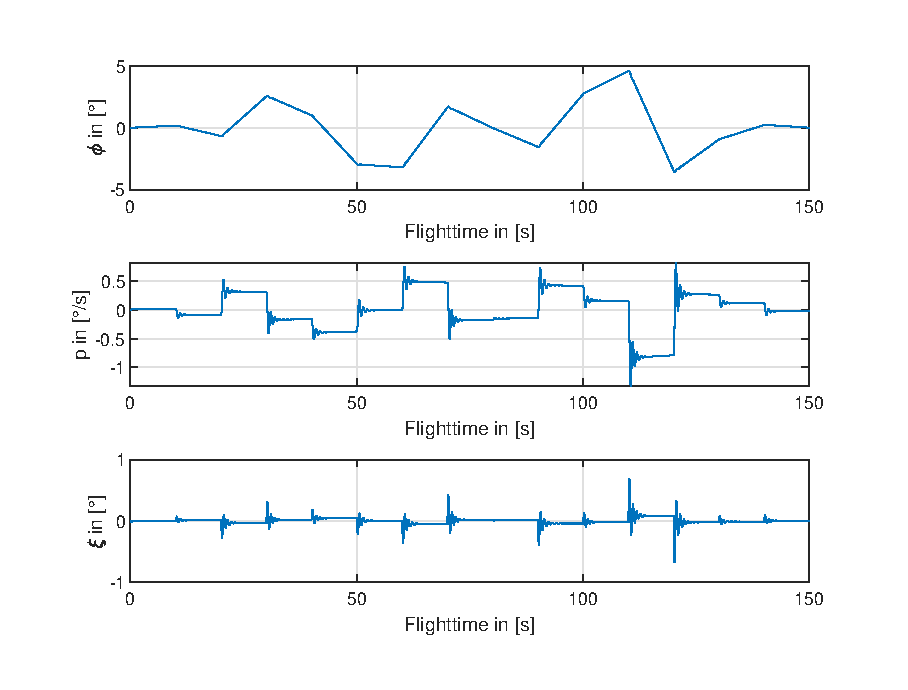
\includegraphics[width=1.0\linewidth]{roll}
\end{minipage}
\begin{minipage}{0.01\linewidth}
	\hfill
\end{minipage}
\begin{minipage}{0.49\linewidth}
	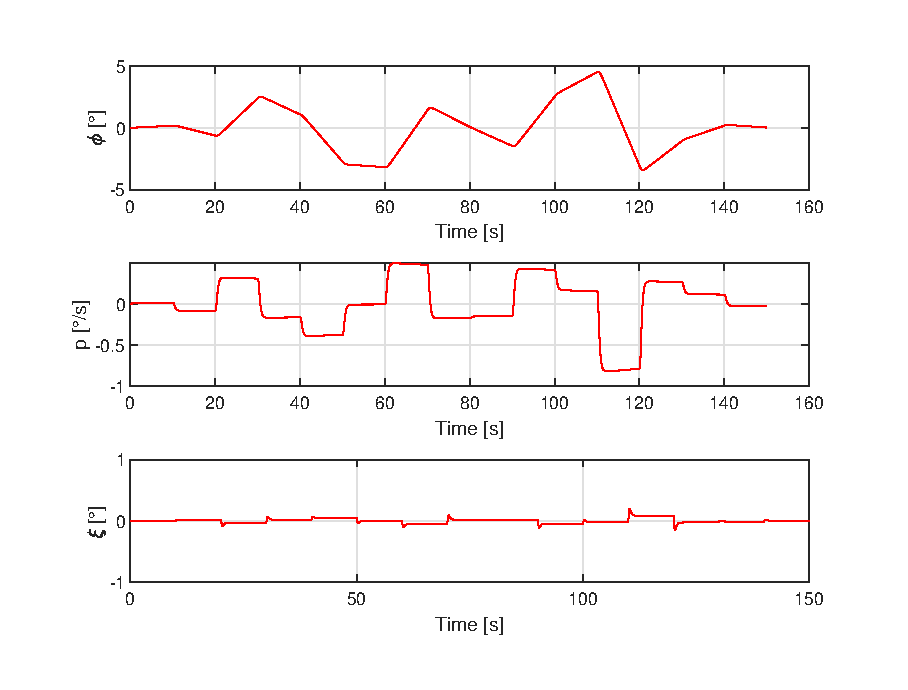
\includegraphics[width=1.0\linewidth]{roll_mat}
\end{minipage}
\captionof{figure}{Vergleich der Seitenbewegung (Rollen), links C++, rechts Matlab}\noindent\\
%
%
\begin{minipage}{0.49\linewidth} 	
	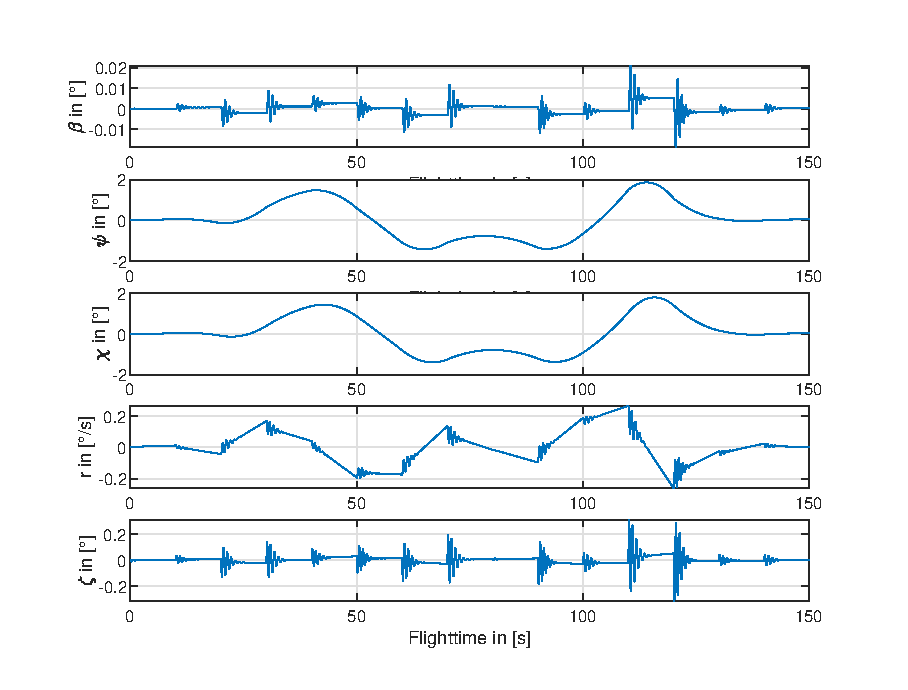
\includegraphics[width=1.0\linewidth]{yaw}
\end{minipage}
\begin{minipage}{0.01\linewidth}
	\hfill
\end{minipage}
\begin{minipage}{0.49\linewidth}
	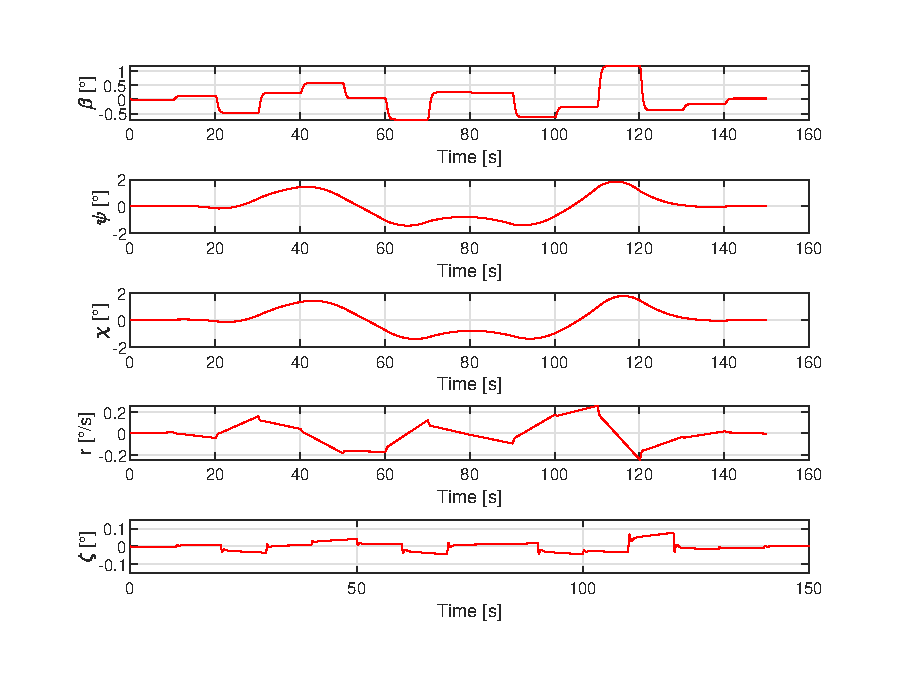
\includegraphics[width=1.0\linewidth]{yaw_mat}
\end{minipage}
\captionof{figure}{Vergleich der Seitenbewegung (Gieren), links C++, rechts Matlab}\noindent\\
%
%
\begin{minipage}{0.49\linewidth} 	
	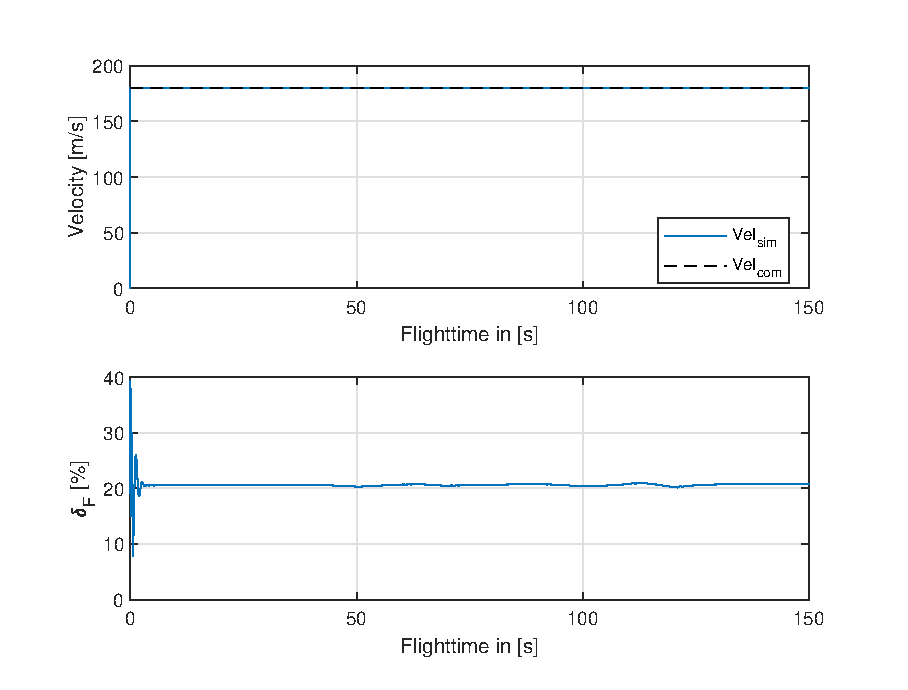
\includegraphics[width=1.0\linewidth]{vel}
\end{minipage}
\begin{minipage}{0.01\linewidth}
	\hfill
\end{minipage}
\begin{minipage}{0.49\linewidth}
	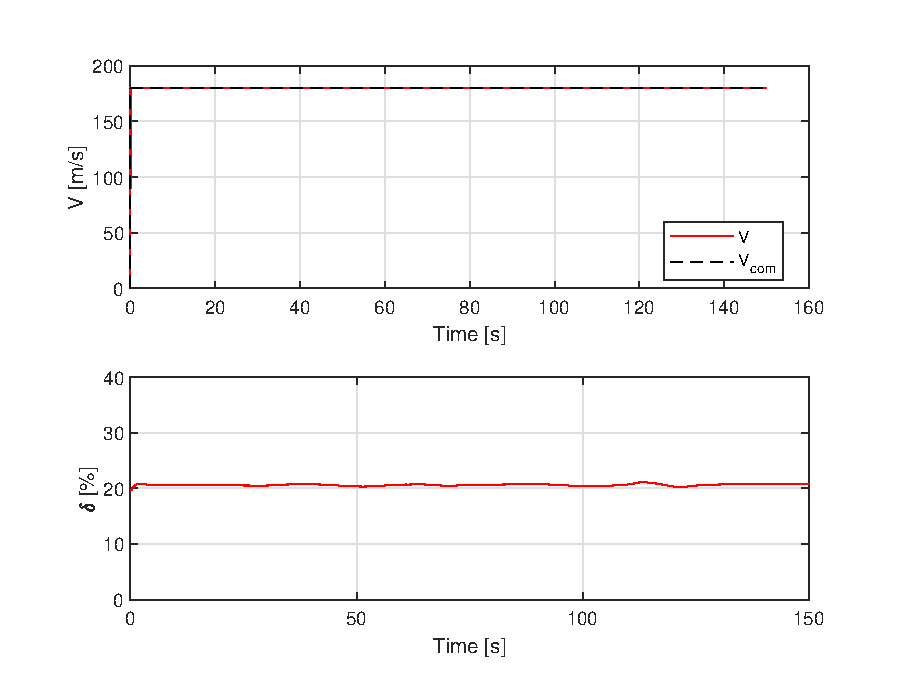
\includegraphics[width=1.0\linewidth]{vel_mat}
\end{minipage}
\captionof{figure}{Vergleich der Geschwindigkeit, links C++, rechts Matlab}\noindent\\

\section{Übersicht Dokumente}
Neben diesem Abschlussbericht, der das Vorgehen und den Aufbau der Simulation erläutern soll, sind im Ordner Documents noch weitere Dokumente hinterlegt. Diese sollen dem Nutzer bei der Bedienung unterstützen.\\
\dirtree{%
	.1 Documents.
	.2 User Manuel.
	.2 Algorithm Description Document.
	.2 Abschlussbericht.
}

%\printbibliography
\newpage
\bibliography{Quelle}

\end{document}